\chapter{Einleitung}
\label{chap:Einleitung}
Mit der fortschreitenden Entwicklung multidisziplinärer Systeme und der Digitalisierung des Maschinen- und Anlagenbaus nimmt die Komplexität des Entwicklungsprozesses zu. Es müssen verschiedene Domänen in einem Produkt integriert und aufeinander abgestimmt werden bei möglichst effizienter Kostenstruktur und Terminplanung. Zugleich bieten Weiterentwicklungen der Modellierungs- uns Simulationssysteme neue Möglichkeiten zur virtuellen Produktentwicklung und Erprobung der Systeme vor deren physischen Realisierung. Begegnet wird der Komplexität des Entwicklungsprozesses durch Nutzung dieser neuen Möglichkeiten in der modellbasierten Systementwicklung. Im Zentrum der Entwicklung steht das Modell, der Digitale Zwilling des Systems, mit dem alle relevanten Informationen und Anforderungen verknüpft sind. An dem Modell können schon in der Entwurfsphase Analysen vorgenommen und zur Verbesserung des Systems verwendet werden. 

Ein Anwendungsgebiet für die modellbasierte Systementwicklung ist die Verknüpfung der Auslegung elektrischer Maschinen mit der Reglerentwicklung und -einstellung. Die Regelung elektrischer Maschinen geschieht häufig mit dem Einsatz von PI- bzw. PID-Reglerstrukturen. Das Einstellen der Reglerparameter wird dabei, sofern kein selbsteinstellender Regler
(Autotuning) verwendet wird, manuell und mit Hilfe von Erfahrungswerten oder Einstellregeln durchgeführt. Dazu muss zuerst die zu regelnde Maschine existieren; die Anpassung des Reglers kann daher erst nach Entwicklung der Anlage, mit der Produktion eines ersten Prototypen erfolgen. Durch den Einsatz der modellbasierten Systementwicklung kann dieser Prozess schon zeitnah mit der elektrischen Auslegung erfolgen. Die dazu nötige Modellbildung, Validierung und eine mögliche Anwendung des Modells sollen im Rahmen dieser Arbeit am Beispiel eines rotierenden Frequenzumformers behandelt werden.

\section{Zielsetzung}
\label{sec:Zielsetzung}
Zunächst soll in dieser Arbeit das Gesamtsystem „rotierender Frequenzumformer“ hinsichtlich Informations- und Energiefluss dokumentiert werden, um einen Überblick über das System zu geben. Im Anschluss soll ein Modell des Systems aufgestellt, simuliert und zur Charakterisierung des Systems eingesetzt werden. Die Vorgehensweise zeigt das Struktogramm in \cref{fig:StrukturArbeit}.   Die Modellierung geschieht auf Grundlage der technischen Daten aus der Auslegung der Anlage und soll so erfolgen, dass eine möglichst große Wiederverwendbarkeit der Modelle für weitere Untersuchungen und Optimierungen ermöglicht wird.  Gegebenenfalls müssen die Daten umgerechnet werden. Nachdem das Modell mit Parametern versehen wurde, wird es verifiziert und mittels Messungen an einer realen Maschine validiert. Anschließend wird das Modell verwendet, um eine Parameterstudie und eine Trendanalyse zum Einfluss der Maschinen- und Reglerparameter durchzuführen. 
\begin{figure}
	\centering
	\input{Tikz-Bilder/control.tikzstyles}
\tikzstyle{load jump}=[block, path picture={
    % Axes
    \node[block axes]{};
    % Plot function
    \draw[thick] plot[smooth] coordinates {%
    (-.4,.2) (-.3,.2) (-.2,.2) (-.18,-.1) (-.16,-.1) (-.08,.2) (0,.2) (.45,.2)
    };
}]
\tikzstyle{ises}=[block, path picture={
    % Axes
    \node[block axes]{};
    % Plot function
    \draw[thick] plot[smooth] coordinates {%
    (-.3,.2) (-.1,-.15) (.3,-.22) 
    };
    %\draw[thick] plot[smooth] coordinates {%
    %(-.3,-.3) (-.1,-.28) (.3,-.05) 
    %};
}]
\tikzstyle{trends}=[block, path picture={
    % Axes
    \draw[thick] ++(-0.4,-0.3) +(0,.6) |- +(.3,0) ++(.5,0) +(0,.6) |- +(.3,0);
    % Plot function
    \draw[mark=x, only marks, mark size=1pt] plot coordinates {
        % Left side
        (-.25,-.25)
        (-.3,-.15)
        (-.2,-.15)
        (-.25,-.05)
        (-.25,.05)
        % Right side
        (.25, -.15)
        (.2, -.1)
        (.3, -.1)
        (.25, 0)
        (.25, .2)
    };
}]

\begin{tikzpicture}[node distance=2cm]
% Nodes
    \node [input, label={left:Daten}] (input) at (0,0) {};
    \node [wide block] (formula) [right of=input] {Umrechnung};
    \node [knot] (knot1) [right of=formula] {};
    
    \node [wide block] (model) [node distance=2cm, right of=knot1] {Modell};
    \node [wide block] (measurement) [below of=model] {Messung};
    
    \node [] (sweeps) [node distance=3cm, right of=model] {};
    \node [load jump, yshift=.1cm, xshift=.1cm] (sweep1) at (sweeps) {};
    \node [load jump] (sweep2) at (sweeps) {};
    \node [load jump, yshift=-.1cm, xshift=-.1cm] (sweep3) at (sweeps) {};
    \node [between=model.east and sweep3.west] (model_sweep) {};
    
    \node [] (ises) [right of=sweeps] {};
    \node [ises, yshift=.1cm, xshift=.1cm] (ise1) at (ises) {};
    \node [ises] (ise2) at (ises) {};
    \node [ises, yshift=-.1cm, xshift=-.1cm] (ise3) at (ises) {};
    
    \node [trends] (trends) [right of=ises] {};

%% Brace + Decoration
    \draw [thick, decorate, decoration = {brace, raise=25pt, amplitude=5pt, mirror}] (sweep3.west |- sweeps.west) -- (trends.east) node[pos=0.5,above=-50pt] {Auswertung};
    
%% Edges
    \draw [signal] (input) -- (formula) -- (knot1);
    \draw [signal] (knot1) -- (model);
    \draw [signal] (measurement) -| (knot1);
    \draw [signal] (model) -- (sweep3.west|-sweeps);
    \draw [signal] (sweep1.east|-sweeps) -- (ise3.west|-ises);
    \draw [signal] (ise1.east|-ises) -- (trends);
    \draw [signal] (model_sweep|-sweeps) |- (measurement);

\end{tikzpicture}
	\caption{Vorgehensweise: Umrechnung der Daten, Modellierung, Vergleich mit Messung, Parameterstudie, Parametertrend}
	\label{fig:StrukturArbeit}
\end{figure}
Die zentralen Fragen, die in dieser Arbeit beantwortet werden sollen, sind daher:
\begin{itemize}
\item Mit welchen Komponenten muss ein Modell aufgebaut werden, um hinreichend genau die reale Maschine abzubilden?
\item Welche Parameter aus der Auslegung der Maschine werden für die Simulation benötigt und wie müssen sie gegebenenfalls umgeformt werden?
\item Wie kann die Gültigkeit des Modells überprüft werden?
\item Welche Erkenntnisse können mit dem Modell gewonnen werden? Welchen Einfluss hat eine Variation der Maschinen- und Regelparameter auf das dynamische Verhalten der Maschine?
\end{itemize}

\section{Überblick über das System rotierender Frequenzumformer}
\label{sec:Uberblick}
Bei der hier betrachteten elektrischen Anlage handelt es sich um den rotierenden Frequenzumformer „Apojet AJR 90“ (siehe \cref{fig:RenderbildUmformer}) der Firma \textsc{Piller Power Systems}. Aufgabe des Frequenzumformers ist es, die durch Energieversorger bereitgestellte \unit[50]{Hz} Netzspannung in ein \unit[400]{Hz} Spannungsystem umzuformen, wie es unter anderem in der Bodenstromversorgung der zivilen und militärischen Luftfahrt zum Einsatz kommt.
Zur Umformung der Netzfrequenz haben sich zwei technische Prinzipien auf dem Markt etabliert. Zum einen werden sogenannte \emph{statische} Umformer eingesetzt, die die Frequenz mit dem Einsatz von Leistungselektroniken umwandeln, und andererseits werden \emph{rotierende} Umformer wie der hier betrachtete eingesetzt. Die rotierenden Umformer realisieren die Frequenzumwandlung durch die Kopplung eines Elektromotors mit einem geeigneten Synchrongenerator anderer Polpaarzahl. Zusammen mit der Frequenz findet auch eine Wandlung der Spannung statt, die über einen Spannungsregler konstant gehalten wird. \cref{tab:Leistungsdaten} gibt einen Überblick über die wichtigsten Technischen Daten.

\begin{figure}
\centering
\begin{subfigure}{.49\textwidth}
	\centering
	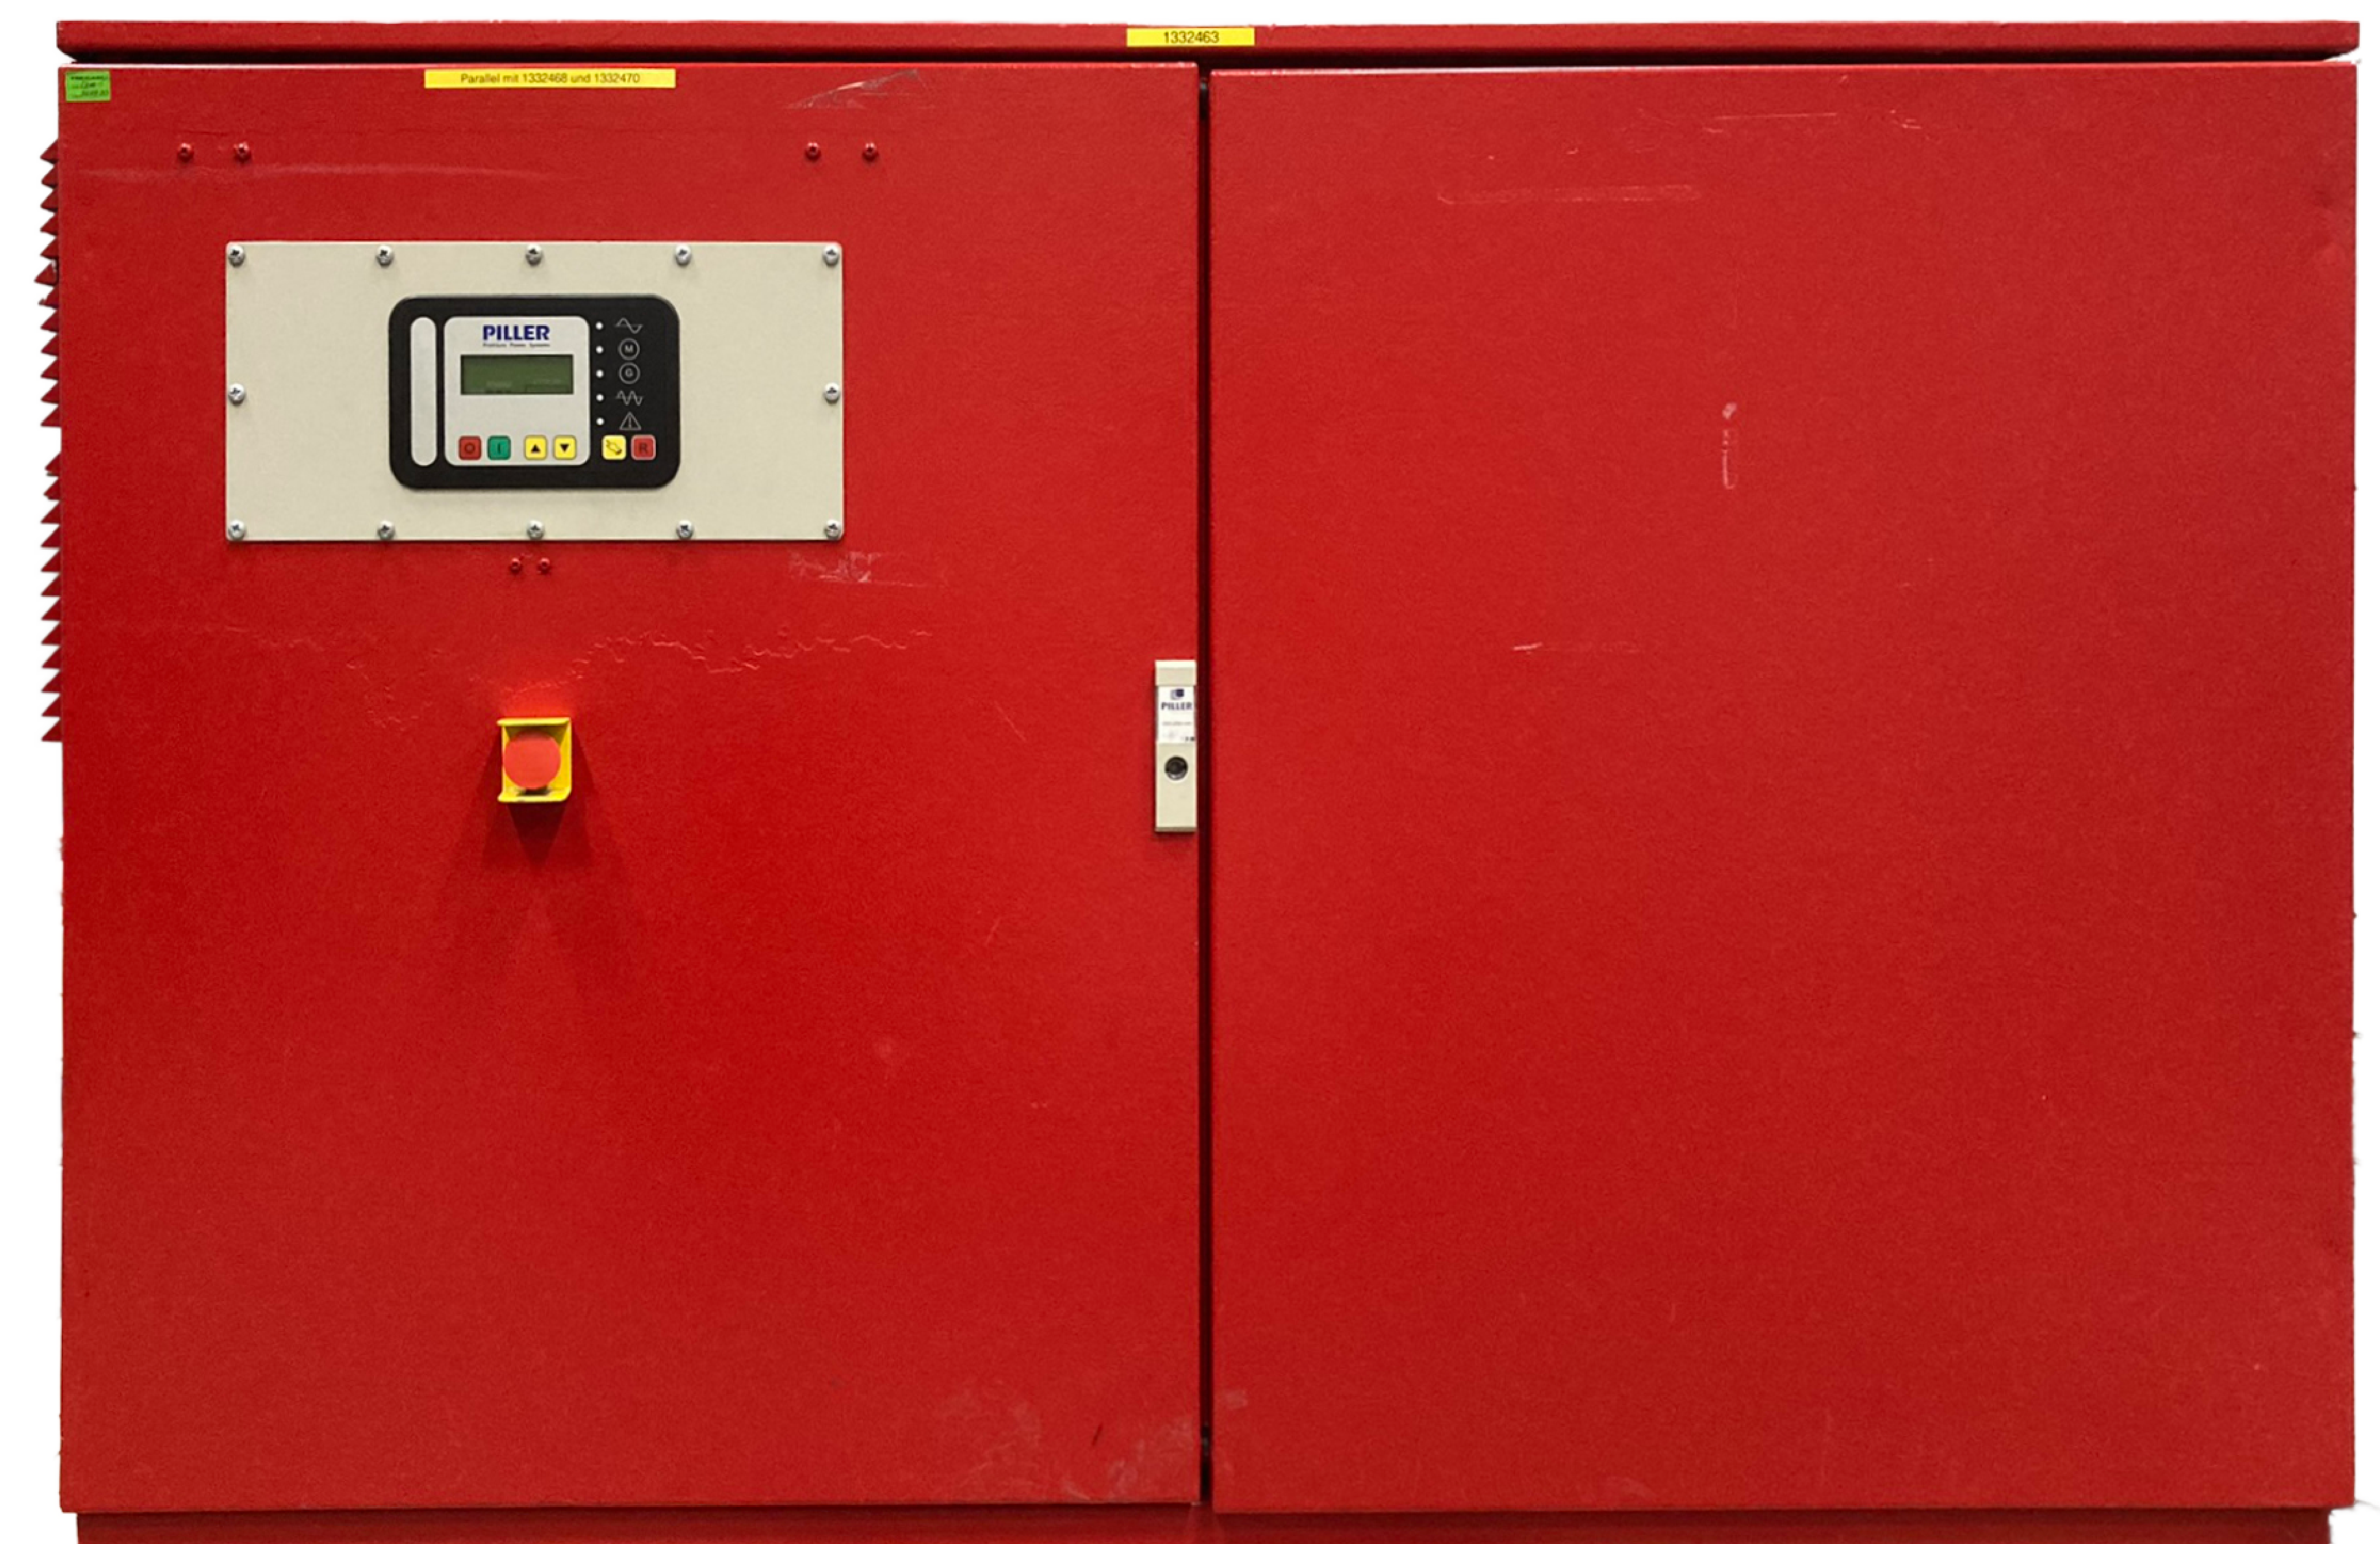
\includegraphics[width=\textwidth]{Bilder/Umformer_vorne_geschlossen.pdf}
	\caption{geschlossene Ansicht}
\end{subfigure}
\begin{subfigure}{.49\textwidth}
	\centering
	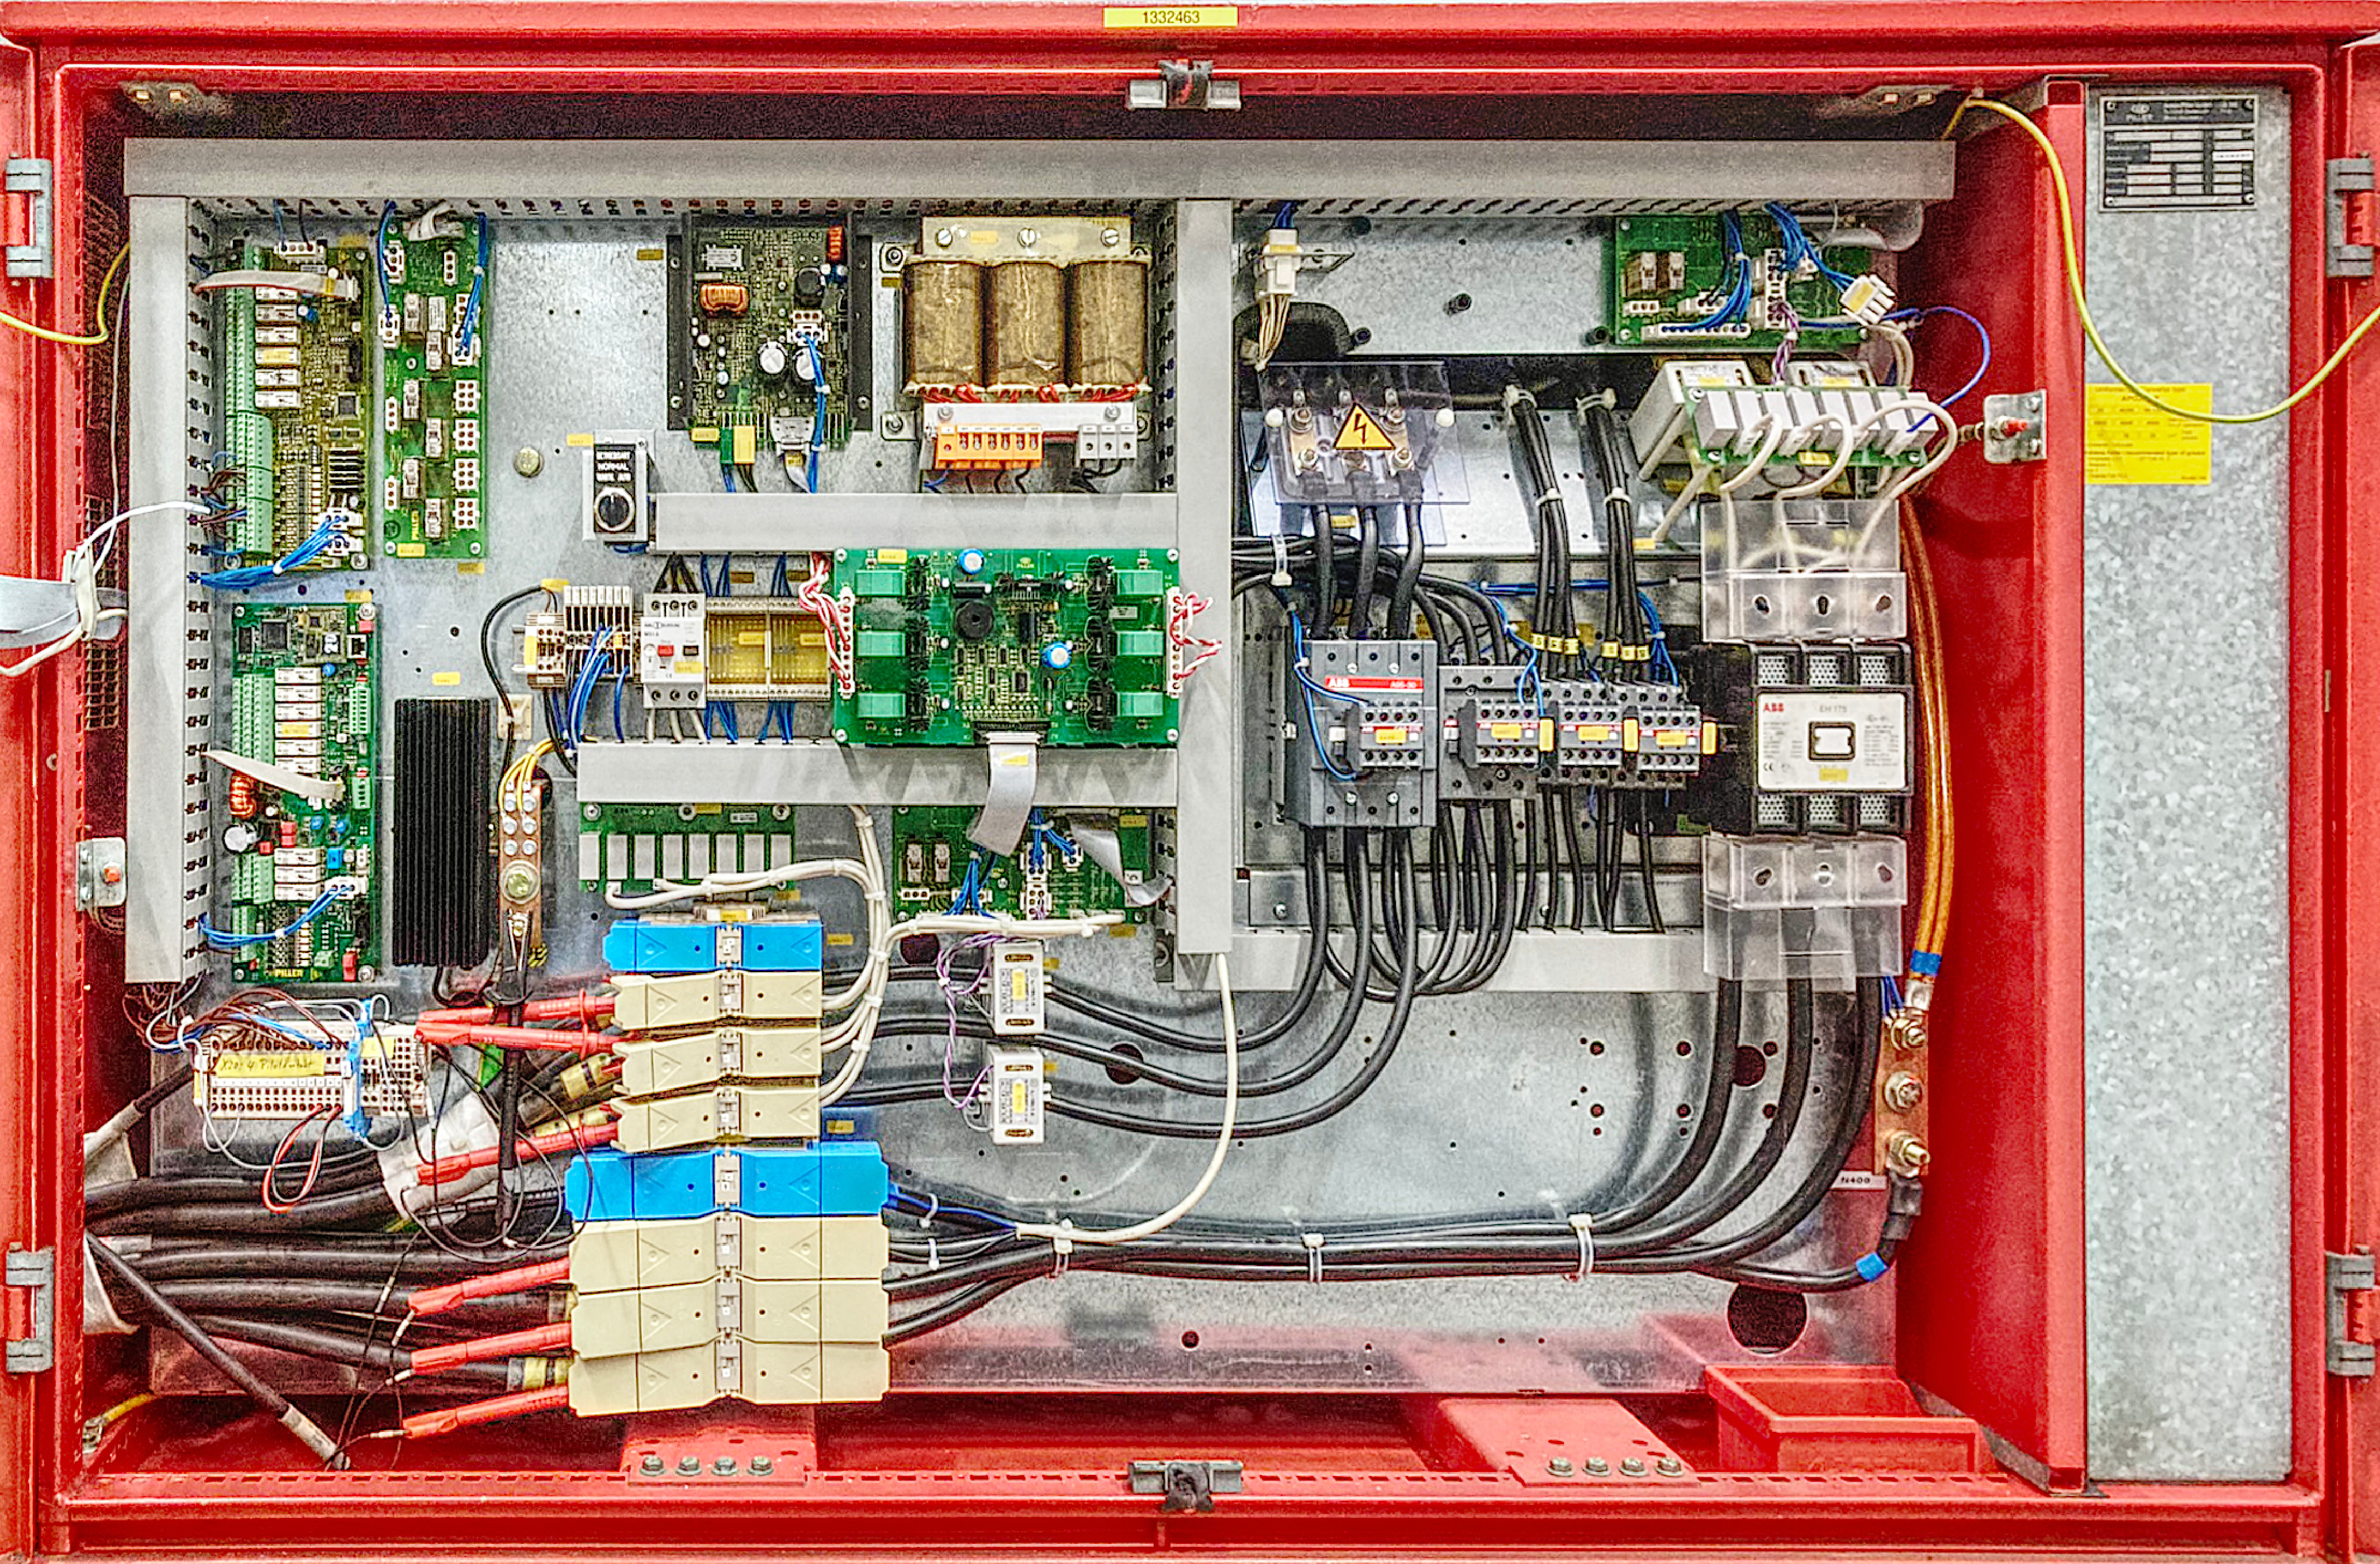
\includegraphics[width=\textwidth]{Bilder/Umformer_vorne_offen.pdf}
	\caption{geöffnete Ansicht}
\end{subfigure}
\caption{Frequenzumformer Apojet AJR 90 (eigene Aufnahmen)}
\label{fig:RenderbildUmformer}
\end{figure}

\begin{table}[b]
\caption{Technische Daten \textsc{Apojet AJR 90} nach \cite{pillerpowersystemsBetriebshandbuchAPOJET202021}}\label{tab:Leistungsdaten}
\centering
\begin{tabular}{@{}ll@{}}
\toprule
Eingang:         & \unit[230/400]{V}, \unit[145]{A}, \unit[50]{Hz}      \\ 
Ausgang:         & \unit[115/200]{V}, \unit[260]{A}, \unit[400]{Hz} \\
Nenndrehzahl:    & $\unit[3000]{\frac{U}{min}}$                     \\
Ausgangsleistung:& 90 kVA, $\mathrm{Pf}=0,8$                        \\
Wirkungsgrad:    & \unit[85]{\%}.                                   \\ \bottomrule
\end{tabular}
\end{table}

